\subsection{Preparation of the Input}

In this section we focus on predicting both real and imaginary parts of the \texttt{exp} label using both the lumps and the \wzw datasets together: the idea is to have a model independent architecture able to make predictions without knowledge of the underlying physical model.

The datasets are however defined differently and many variables differ in the two physical models.
We start from the tidy datasets which have been prepared for the separate analysis in the previous sections.

We will proceed as follows, before merging the datasets:
\begin{itemize}
  \item we define an effective weight $\hat{h}$ in the \wzw model such that $\hat{h} = \abs{h \cdot m}$, where $h$ is the value of the \texttt{weight} variable in the dataset and $m$ is one of the quantum numbers associated with the \SU{2} representation,\footnotemark{}
    \footnotetext{%
      The idea is to have an engineered feature which combines \texttt{k}, \texttt{j} and \texttt{m} in the same range as the \texttt{weight} variable in the lumps dataset.
    }
  \item we transform the columns in the lumps dataset to account for the imaginary parts of the truncation levels (in this dataset they will be identically vanishing),
  \item we compute the PCA of the truncation levels in both datasets, keeping 10 components each to maximise the retained variance,
  \item in the lumps dataset we then select the \texttt{weight}, \texttt{type} and the PCA variables,
  \item in the \wzw dataset we select the effective weight, \texttt{type} and the PCA variables,
  \item we \emph{outer join} the datasets on the \texttt{weight} and \texttt{type} variables.
\end{itemize}
We finally have a new dataset containing 12 features and 2 labels (i.e.\ $\Re(exp)$ and $\Im(exp)$), and 2379 samples.


\subsection{Validation Strategy}

For the analysis we keep \SI{80}{\percent} of the samples for training, \SI{10}{\percent} for validation and \SI{10}{\percent} as a test set as we did before for the two separate datasets.
In this case the datasets can be freely shuffled since all the information on the model is already encoded in the variables.

Before passing the input to the algorithms we scale it using the \texttt{StandardScaler} class in \texttt{Scikit-learn} in order to standardise the features and simplify the learning process.
The labels are not scaled, thus the predictions are directly comparable with the ground truth values.

We focus on predicting both $\Re(exp)$ and $\Im(exp)$ at the same time with a single model.
We will use, as a comparison, the SVM with the Gaussian kernel and an ANN model.
However, since the first cannot naturally account for two outputs, we use the \texttt{MultiOutputRegressor} class in \texttt{Scikit-learn} which automatically uses the same estimator to predict separately both labels.

We will finally provide also the predictions on the double lumps using the trained models to check the ability to generalise to other datasets.


\subsection{Support Vector Machines}

\subsubsection{Training}

The model used for training is a single architecture to predict both real and imaginary parts of \texttt{exp}.
We do not perform any automatic optimisation since the interface with the \emph{Scikit-optimize} Bayes cycle does not allow to predict two labels at the same time.
Moreover hyperparameters chosen for predicting $\Re(exp)$ are in principle different from those used to predict $\Im(exp)$.
We manually choose $C = 10^5$, $\epsilon= 0.1$ and $\gamma = 0.1$ (respectively reffering to the penalty assigned to distant samples, the \emph{no penalty} rigid boundary, and the width of the Gaussian kernel).


\subsubsection{Results}

Results on the test fold are summarised in \Cref{tab:agg:svr_met}.
Even though the algorithm performed well on the validation set ($\mse = 0.09$ for $\Re(exp)$ and $\mse = 0.03$ for $\Im(exp)$), the results on the generalisation set are one order of magnitude larger.
Even though it may be difficult to isolate the cause, it seems the worst result is mainly due to very few samples whose predictions is heavily influecing the bad result, as shown in \Cref{fig:agg:svr_pred}.
We will therefore need to check these predictions, since the algorithm seems to perform quite well otherwise, as the residual plot shows in \Cref{fig:agg:svr_res_plot}.

\begin{table}[htbp]
  \centering
  %\resizebox{\textwidth}{!}{%
  \begin{tabular}{@{}ccccc@{}}
  \toprule
             & \dof & \mse & \mae & \rr   \\
  \midrule
  $\Re(exp)$ & 226  & 0.3  & 0.15 & 0.36  \\
  $\Im(exp)$ & 226  & 0.3  & 0.11 & -3.4  \\
  \bottomrule
  \end{tabular}%
  %}
  \caption{Summary of the metrics of the \emph{r-SVR} on the test set.}
  \label{tab:agg:svr_met}
\end{table}

\begin{figure}[htbp]
  \centering
  \begin{subfigure}{0.45\textwidth}
    \centering
    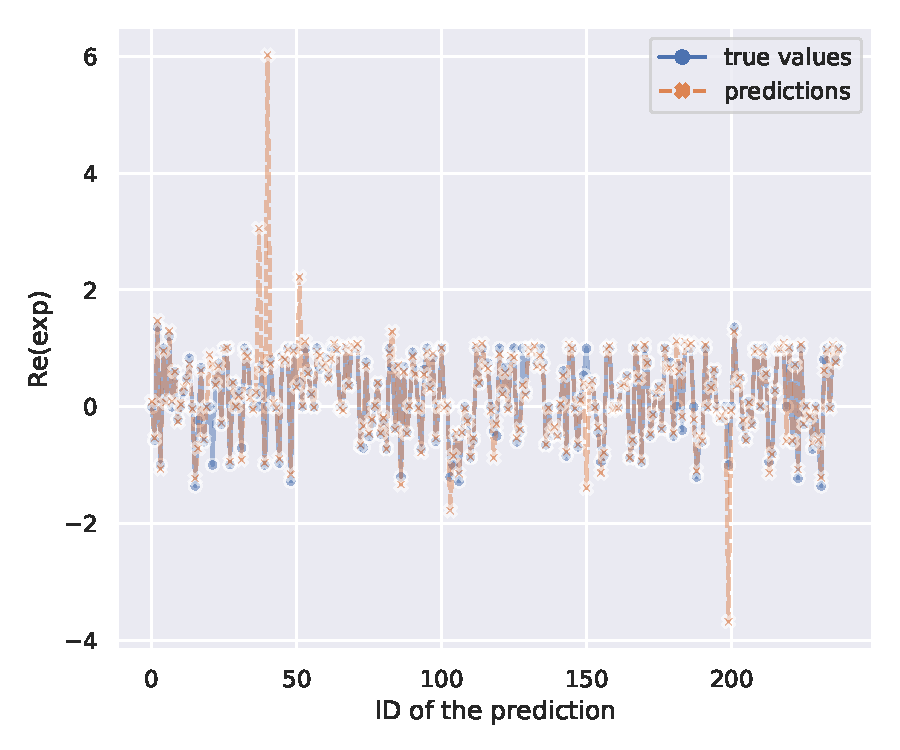
\includegraphics[width=\linewidth]{img/svr_test_exp_re_plot}
    \caption{Real part.}
  \end{subfigure}
  \begin{subfigure}{0.45\textwidth}
    \centering
    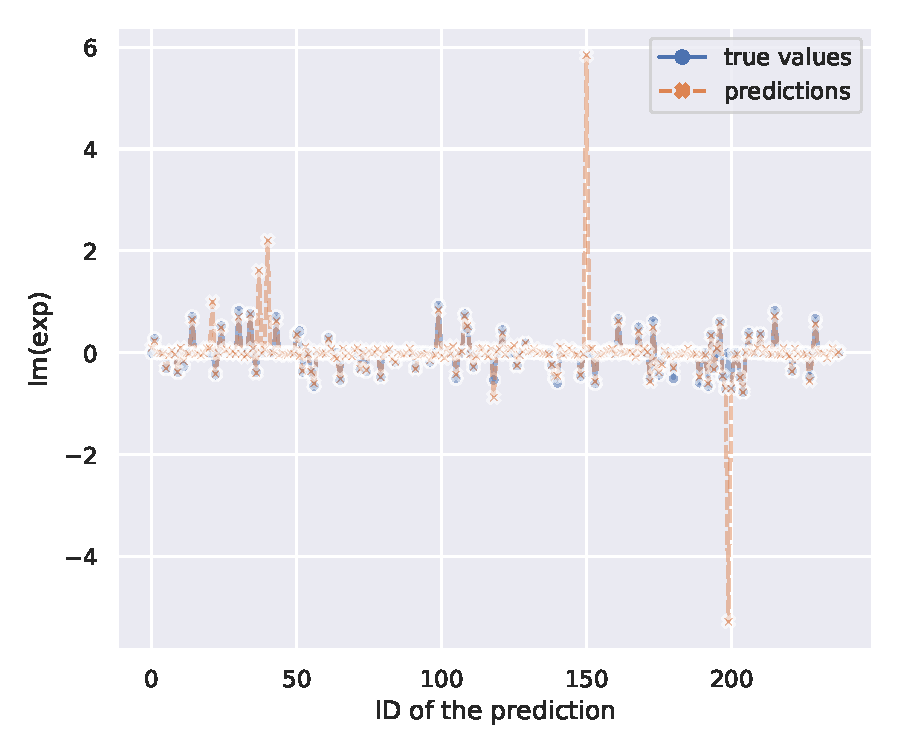
\includegraphics[width=\linewidth]{img/svr_test_exp_im_plot}
    \caption{Imaginary part.}
  \end{subfigure}
  \caption{Predictions and true values using the \emph{r-SVR} algorithm.}
  \label{fig:agg:svr_pred}
\end{figure}

\begin{figure}[htbp]
  \centering
  \begin{subfigure}{0.45\textwidth}
    \centering
    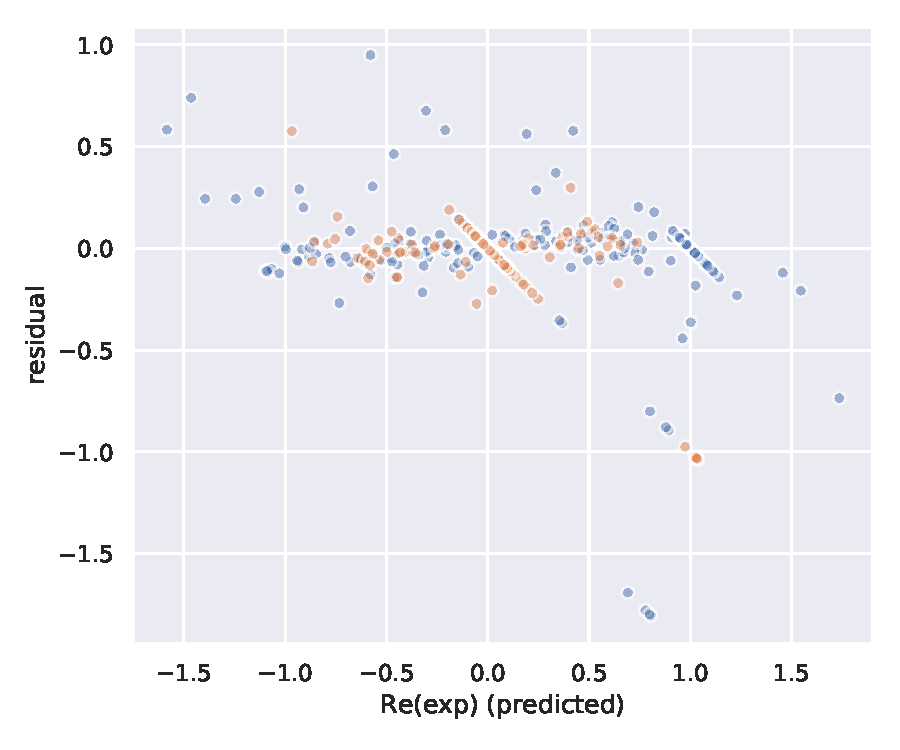
\includegraphics[width=\linewidth]{img/svr_val_res_plot}
    \caption{Validation set.}
  \end{subfigure}
  \begin{subfigure}{0.45\textwidth}
    \centering
    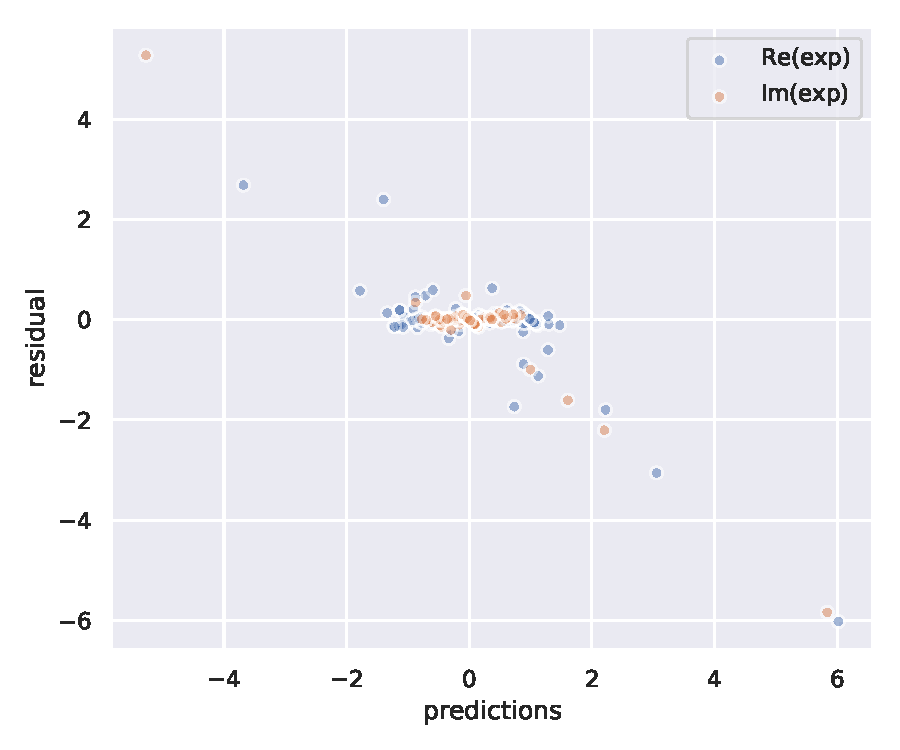
\includegraphics[width=\linewidth]{img/svr_test_res_plot}
    \caption{Test set.}
  \end{subfigure}
  \caption{Residual plot using the \emph{r-SVR}.}
  \label{fig:agg:svr_res_plot}
\end{figure}


\subsection{Artificial Neural Network}

\subsubsection{Model}

The model we use for training is a simple fully connected network (summarised in \Cref{tab:agg:keras_summary}).
The architecture is made of 4 hidden layers with \numlist{30;30;10;10} units each and dropout layers (with rate \num{0.05}) after the first two hidden layers (see \Cref{fig:agg:arch}).
The addition of batch normalisation layers drastically increased the error, so we dropped them entirely in this implementation.

\begin{table}[htbp]
  \centering
  \begin{tabular}{@{}lcc@{}}
    \toprule
    \textbf{layer}           & \textbf{shape} & \textbf{parameters} \\
    \midrule
    \emph{input}             & (12,)          & 0                   \\
    \emph{fully connected}   & (30,)          & 390                 \\
    \emph{dropout}           & (30,)          & 0                   \\
    \emph{fully connected}   & (30,)          & 930                 \\
    \emph{dropout}           & (30,)          & 0                   \\
    \emph{fully connected}   & (10,)          & 310                 \\
    \emph{fully connected}   & (10,)          & 110                 \\
    $\Re(exp)$ (output)      & (1,)           & 11                  \\
    $\Im(exp)$ (output)      & (1,)           & 11                  \\
    \midrule
    \emph{Total parameters:}     & \num{1762}     &                 \\
    \emph{Trainable parameters:} & \num{1762}     &                 \\
    \bottomrule
  \end{tabular}
  \caption{Summary of the network.}
  \label{tab:agg:keras_summary}
\end{table}

\begin{figure}[htbp]
  \centering
  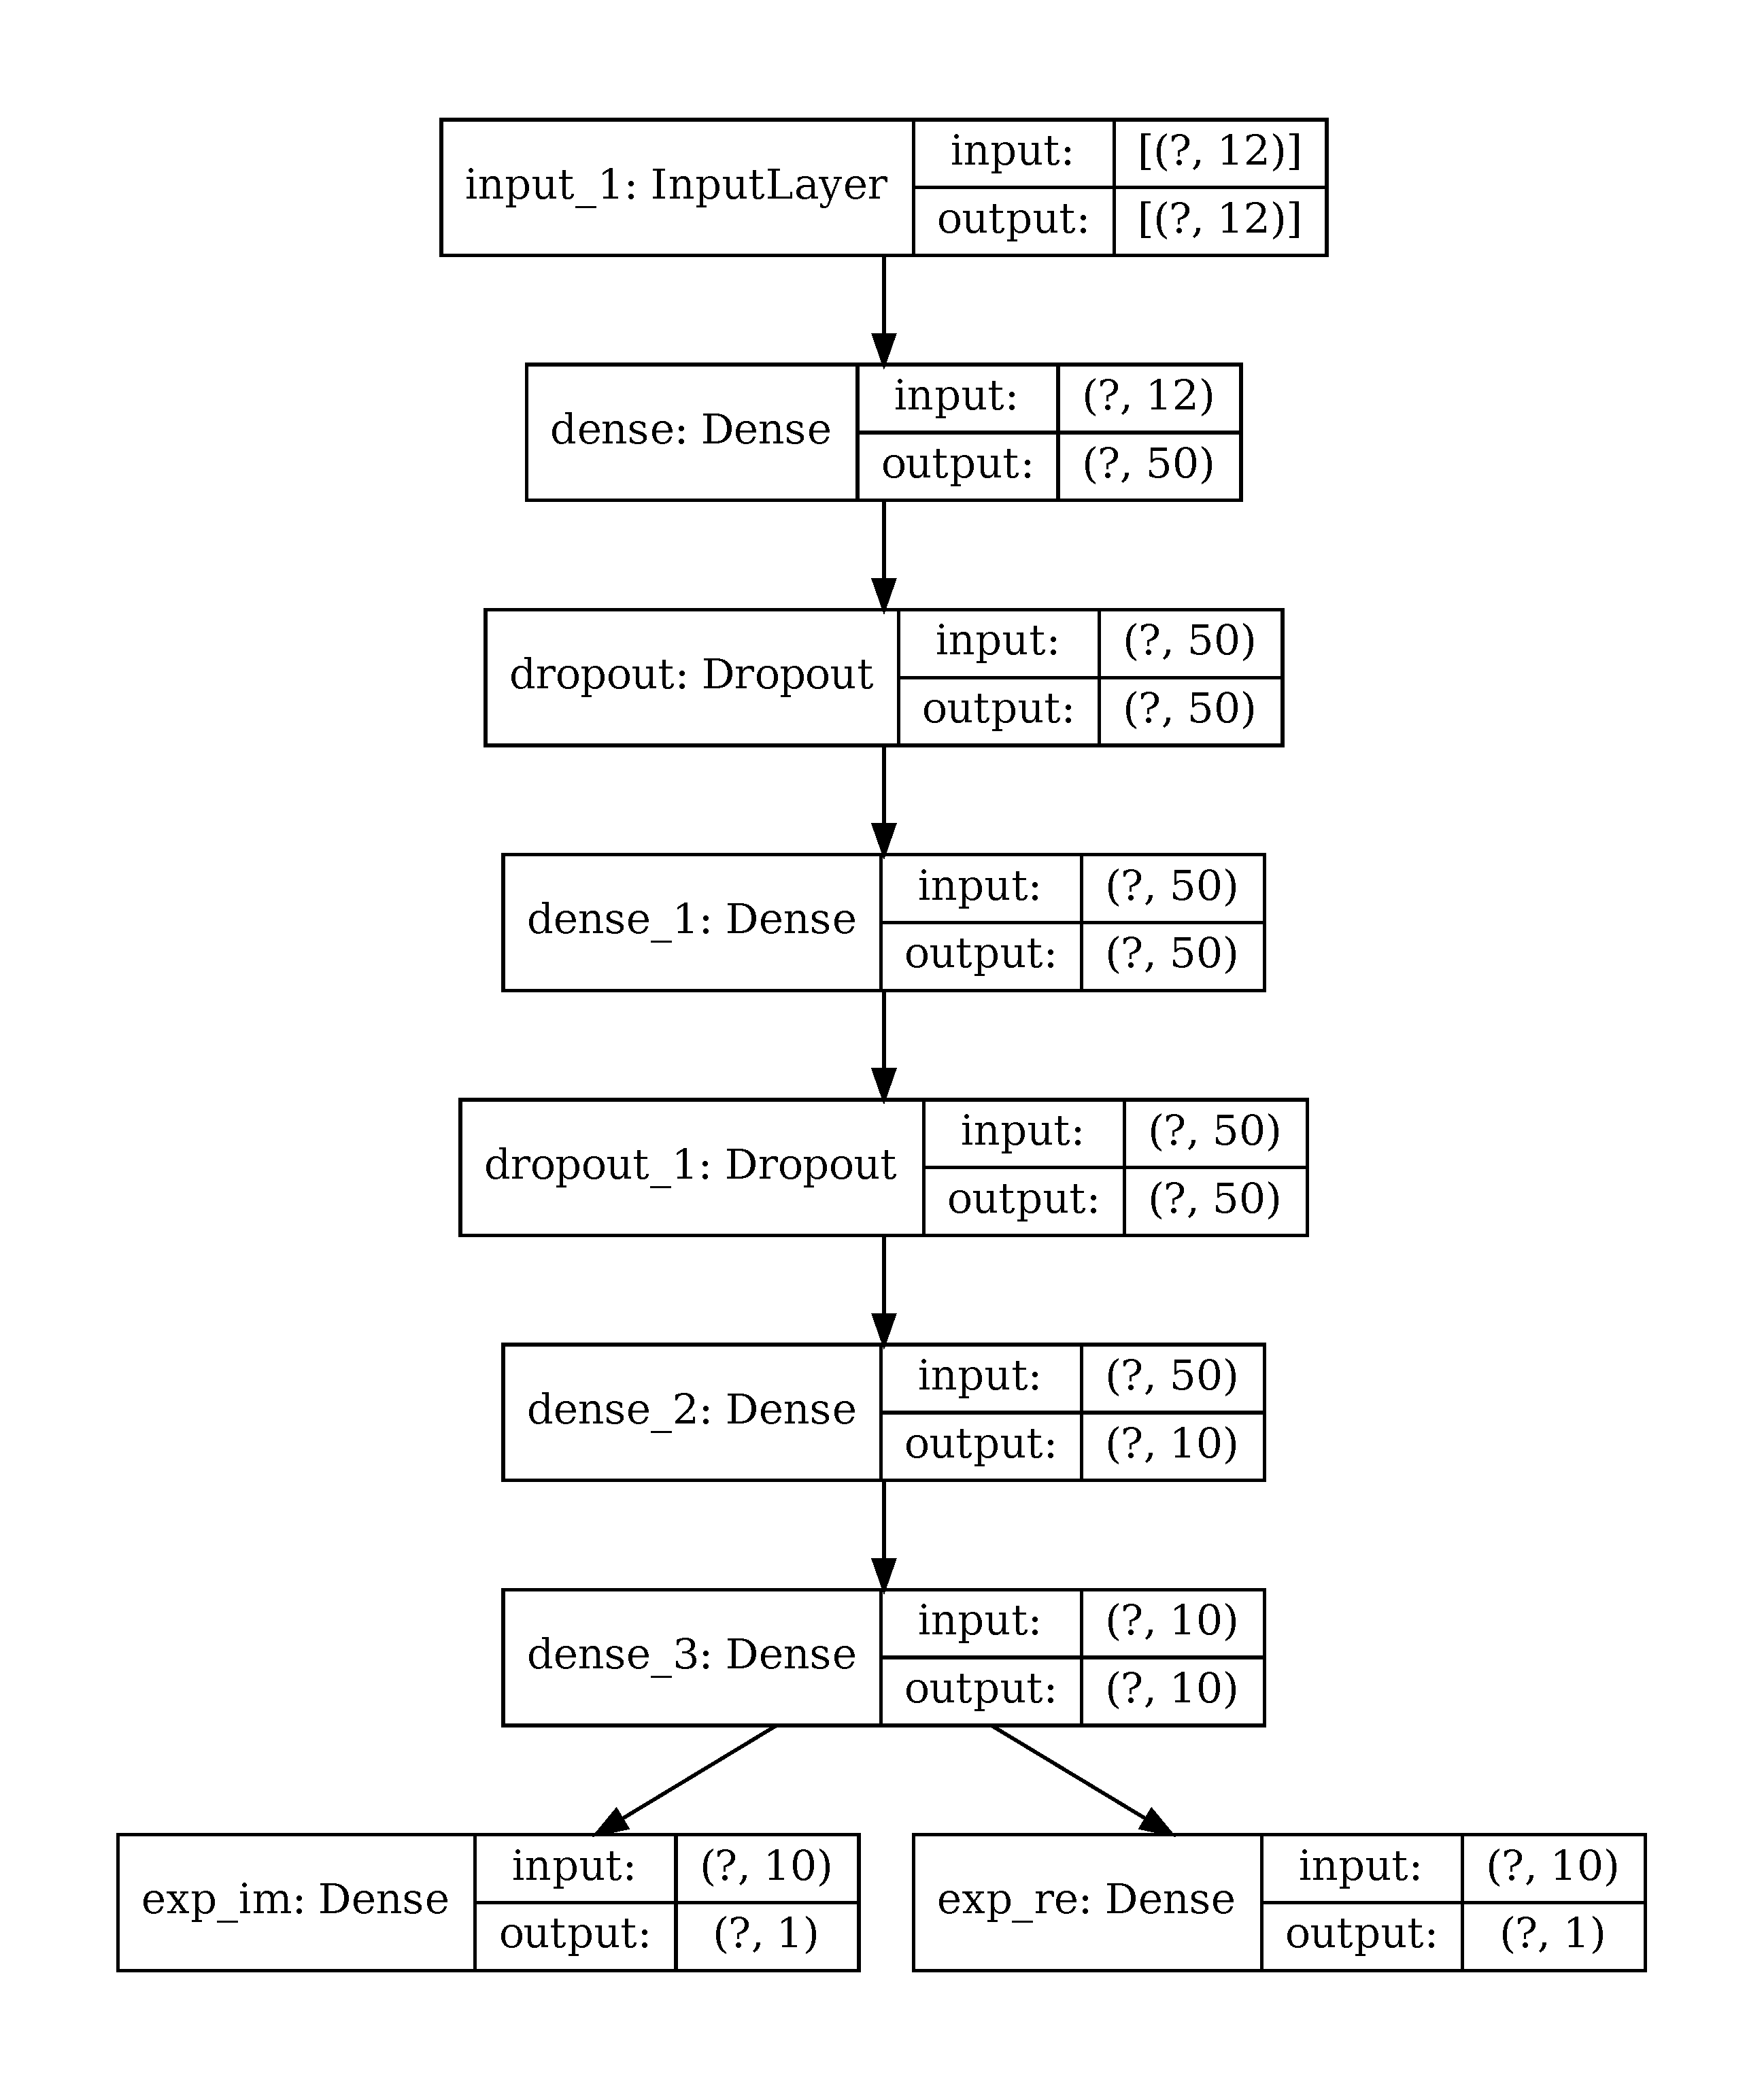
\includegraphics[width=0.6\textwidth]{img/ann_arch}
  \caption{Architecture of the ANN.}
  \label{fig:agg:arch}
\end{figure}


\subsubsection{Training}

For training we use the \mse as loss function and weigh it on the two output layers eavenly with \numlist{0.5;0.5} loss weights.\footnotemark{}
\footnotetext{%
  The loss function must be a scalar metric, thus the \mse in this case is separately computed on the output layers and then combined using the loss weights by multiplying each loss by its weight.
}
For gradient descent we use the \emph{Adam} optimiser with default values and initial learning rate of \num{0.001} and a mini batch size of 32.
The maximal number of epochs used for training is \num{20000} but it greatly exceeds what actually needed for good results.
In fact we also implement a callback to early stop the training after 1000 epochs without improvement of the loss function on the validation data.
We finally add a callback to reduce the learning rate by a step factor of \num{0.3} after 750 epochs without improvement on the validation loss.

The loss function and the \mse are displayed in log scale in \Cref{fig:agg:err}.
They show a drastic drop in error and loss around 100 epochs of training and a stabilisation after that.
Early stopping the network has also the regularisation effect of avoiding the overfit of the traning set.

\begin{figure}[htbp]
  \centering
  \begin{subfigure}{0.45\textwidth}
    \centering
    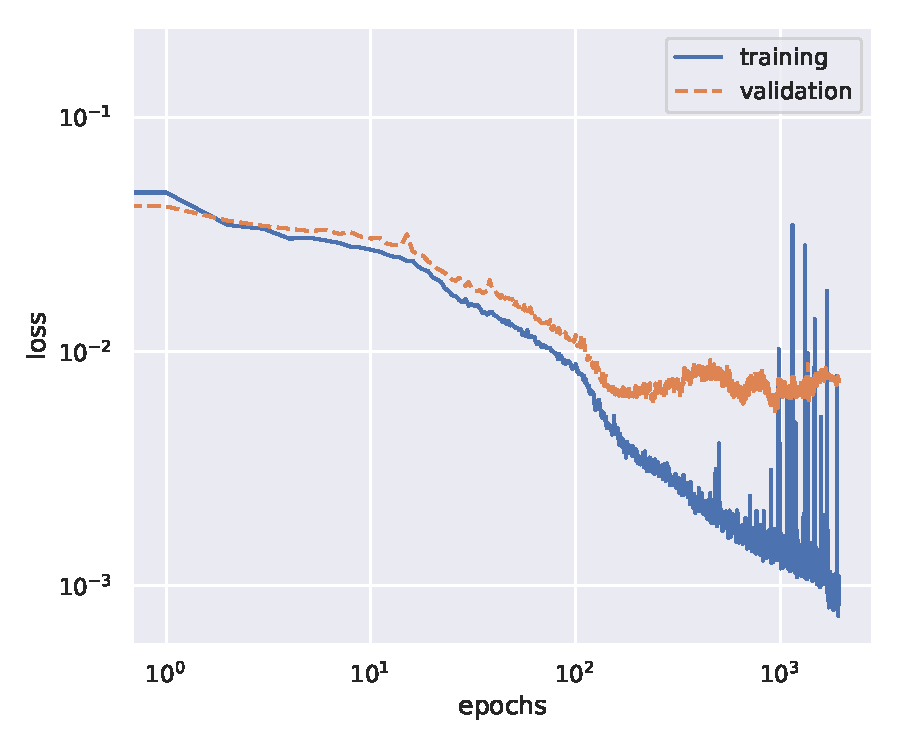
\includegraphics[width=\linewidth]{img/loss}
    \caption{Loss.}
  \end{subfigure}
  \begin{subfigure}{0.45\textwidth}
    \centering
    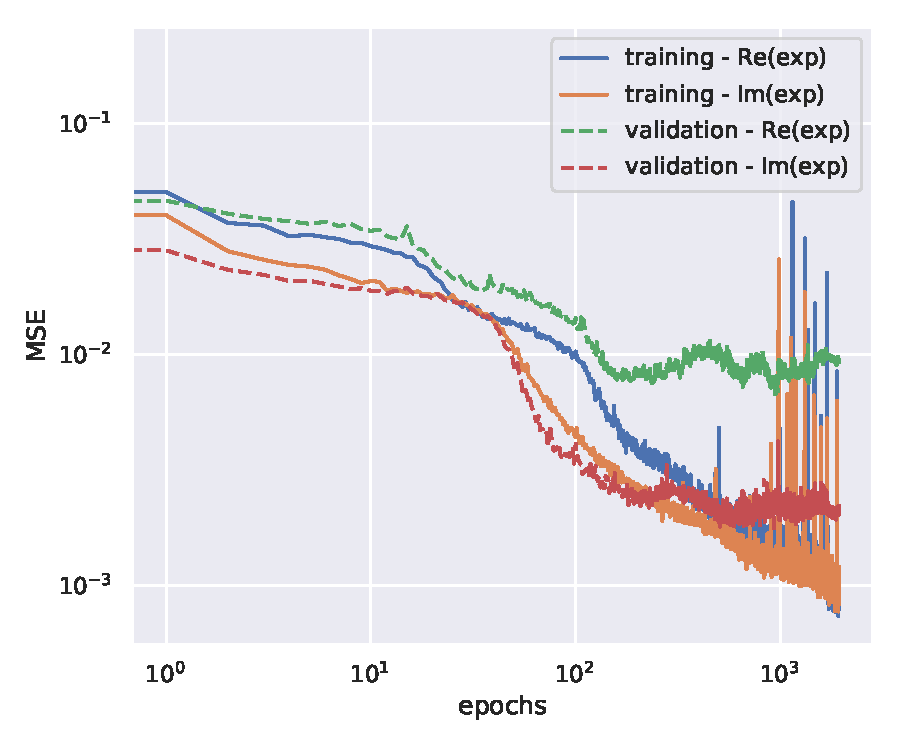
\includegraphics[width=\linewidth]{img/mse}
    \caption{\mse.}
  \end{subfigure}
  \caption{Loss function and errors (log scale).}
  \label{fig:agg:err}
\end{figure}


\subsubsection{Results}

The metrics computed on the test set are shown in \Cref{tab:agg:ann_metrics}.
The results are in general good and the coefficient of determination \rr is very high for both labels.
Comparing with the results in the validation set ($\rr = 0.94$ for $\Re(exp)$ and $\rr = 0.95$ for $\Im(exp)$), it seems that the architecture does not overfit the validation set.\footnotemark{}
\footnotetext{%
  This is in general a risk when using a single validation set.
}

\begin{table}[htbp]
  \centering
  %\resizebox{\textwidth}{!}{%
  \begin{tabular}{@{}ccc@{}}
  \toprule
       & $\Re(exp)$ & $\Im(exp)$ \\
  \midrule
  \mse & 0.02       & 0.002      \\
  \mae & 0.09       & 0.03       \\
  \rr  & 0.96       & 0.96       \\
  \bottomrule
  \end{tabular}%
  %}
  \caption{Metrics of the ANN computed on the test set.}
  \label{tab:agg:ann_metrics}
\end{table}

In fact, \Cref{fig:agg:ann_preds} shows that the agreement between predictions and true values in the test set is very good.
It also does not show signs of isolated samples producing a completely wrong predictions as for the \emph{r-SVR}.
Taking a look at the residuals we can also see that the errors are in general well distributed and do not show sign of patterns (see \Cref{fig:agg:ann_res}).

\begin{figure}[htbp]
  \centering
  \begin{subfigure}{0.45\textwidth}
    \centering
    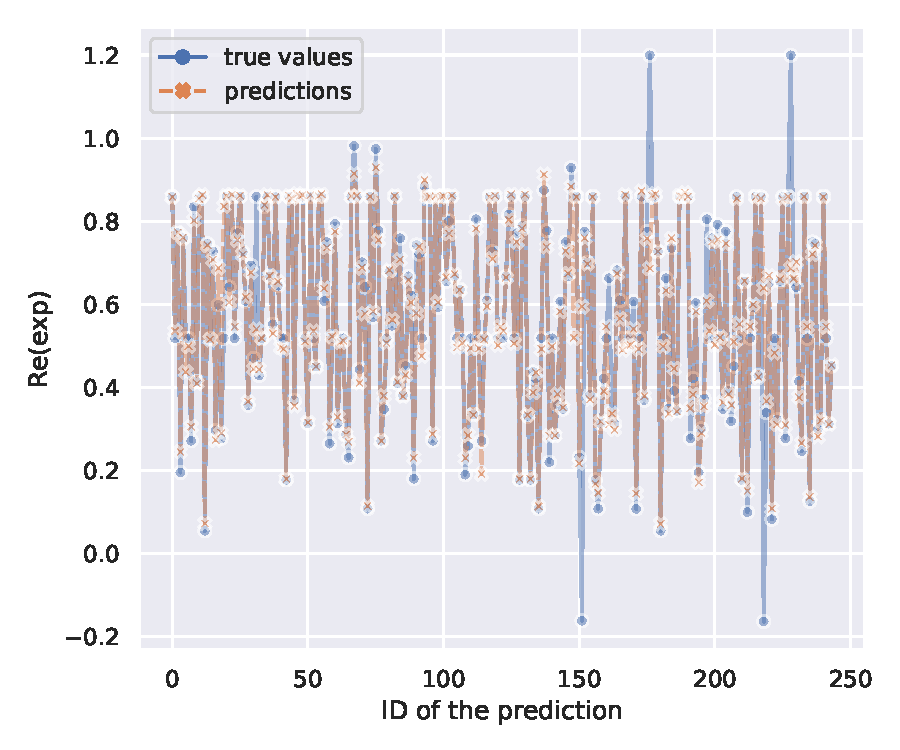
\includegraphics[width=\linewidth]{img/test_exp_re_plot}
    \caption{Real part.}
  \end{subfigure}
  \begin{subfigure}{0.45\textwidth}
    \centering
    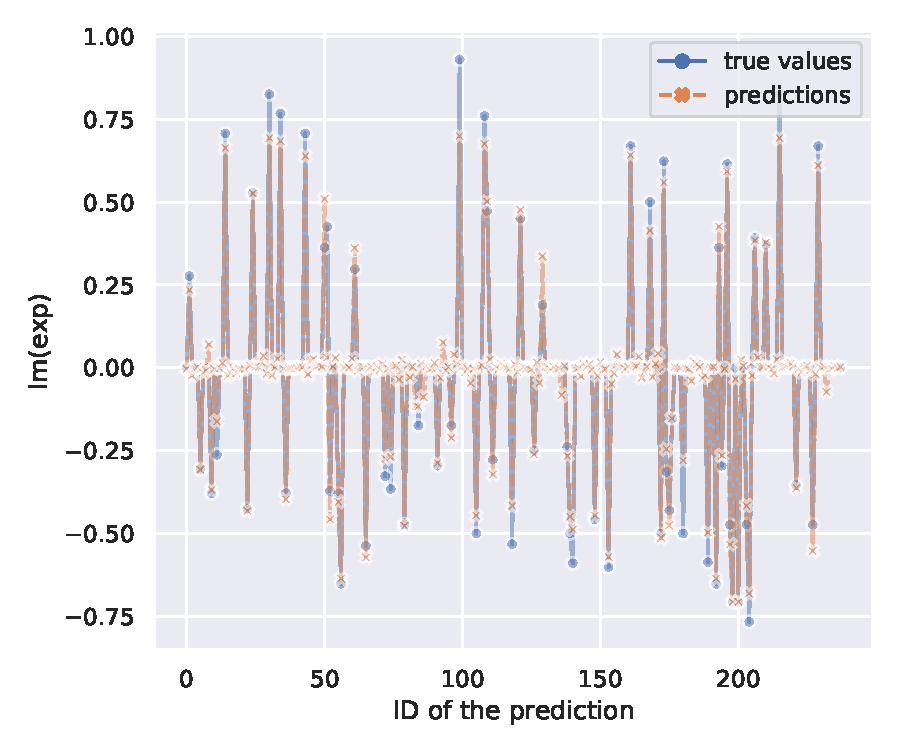
\includegraphics[width=\linewidth]{img/test_exp_im_plot}
    \caption{Imaginary part.}
  \end{subfigure}
  \caption{Predictions and true values using the \emph{ANN} model.}
  \label{fig:agg:ann_preds}
\end{figure}

\begin{figure}[htbp]
  \centering
  \begin{subfigure}{0.45\textwidth}
    \centering
    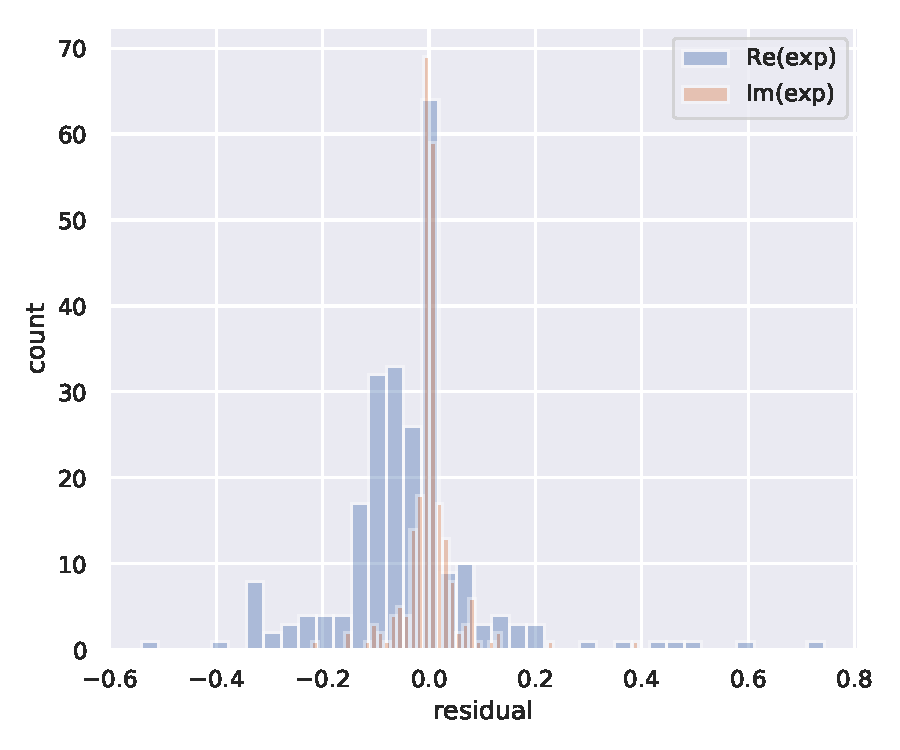
\includegraphics[width=\linewidth]{img/test_res_dist}
    \caption{Univariate distribution.}
  \end{subfigure}
  \begin{subfigure}{0.45\textwidth}
    \centering
    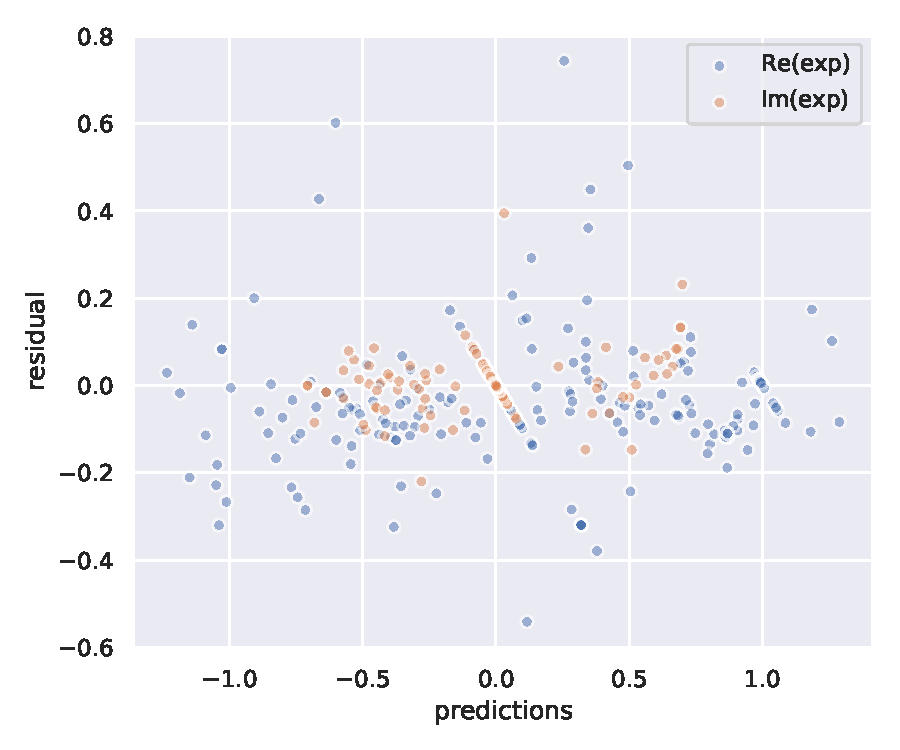
\includegraphics[width=\linewidth]{img/test_res_plot}
    \caption{Residual plot.}
  \end{subfigure}
  \caption{Residuals of the \emph{ANN} model.}
  \label{fig:agg:ann_res}
\end{figure}


\subsection{Double Lumps}

We finally use the two models trained in this section to compute the predictions on the double lumps.
We then select only the most reliable solutions (i.e.\ \texttt{weight} $< 1.5$) and compute the metrics which are summarised in \Cref{tab:agg:dlumps}.
In general it seems that the \emph{ANN} performed better even though the results are far from good.

\begin{table}[htbp]
  \centering
  \resizebox{\textwidth}{!}{%
  \begin{tabular}{@{}ccccccc@{}}
  \toprule
        & \mse $\left( \Re(exp) \right)$
        & \mse $\left( \Im(exp) \right)$
        & \mae $\left( \Re(exp) \right)$
        & \mae $\left( \Im(exp) \right)$
        & \rr $\left( \Re(exp) \right)$
        & \rr $\left( \Im(exp) \right)$ \\
  \midrule
  \emph{r-SVR} & 55 & 130   & 4   & 11   & -23   & 0.0 \\
  \emph{ANN}   & 2  & 0.004 & 1.3 & 0.05 & 0.016 & 0.0 \\
  \bottomrule
  \end{tabular}%
  }
  \caption{Metrics computed on the double lumps.}
  \label{tab:agg:dlumps}
\end{table}

Looking directly at the predictions (they are only 12 values) in \Cref{tab:agg:ann_comp}, we can see that the prediction of the real part of \texttt{exp} are in general completely off (an entire order of magnitude of difference).
However the predictions of the imaginary part have all vanishing integer part: assuming knowldge of the reality of \texttt{exp} for this model, we can in principle accept the predictions by simply truncating the results.\footnotemark{}
\footnotetext{%
  The important point is however that the model was trained on a dataset which included complex variables.
  It is not guaranteed to work also on a dataset with only real values.
  We may therefore have to adjust the predictions to account for that.
}

\begin{table}[htbp]
  \centering
  %\resizebox{\textwidth}{!}{%
  \begin{tabular}{@{}cccc@{}}
  \toprule 
  \emph{ANN} $(\Re(exp))$ &
  \emph{ANN} $(\Im(exp))$ &
  $\Re(exp)$ &
  $\Im(exp)$ \\
  \midrule
  -0.11 & 0.03 & 2.00  & 0.00 \\
  0.07  & 0.05 & -0.00 & 0.00 \\
  0.5   & 0.05 & -2.0  & 0.00 \\
  0.6   & 0.02 & 2.0   & 0.00 \\
  0.7   & 0.04 & 1.0   & 0.00 \\
  0.5   & 0.04 & -1.1  & 0.00 \\
  0.3   & 0.15 & -2.0  & 0.00 \\
  0.4   & 0.09 & -0.8  & 0.00 \\
  0.14  & 0.09 & 1.21  & 0.00 \\
  1.0   & 0.03 & 2.0   & 0.00 \\
  0.7   & 0.02 & 0.7   & 0.00 \\
  0.6   & 0.02 & 2.0   & 0.00 \\
  \bottomrule
  \end{tabular}%
  %}
  \caption{Predictions of the \emph{ANN} model.}
  \label{tab:agg:ann_comp}
\end{table}
